% --------------------------------------------------------------
% This is all preamble stuff that you don't have to worry about.
% Head down to where it says "Start here"
% --------------------------------------------------------------
 
\documentclass[12pt]{article}
 
\usepackage[margin=1in]{geometry} 
\usepackage{amsmath,amsthm,amssymb, graphicx}
 \usepackage{algorithm}
\usepackage{algorithmic}

\newcommand{\N}{\mathbb{N}}
\newcommand{\Z}{\mathbb{Z}}
 
\newenvironment{theorem}[2][Theorem]{\begin{trivlist}
\item[\hskip \labelsep {\bfseries #1}\hskip \labelsep {\bfseries #2.}]}{\end{trivlist}}
\newenvironment{lemma}[2][Lemma]{\begin{trivlist}
\item[\hskip \labelsep {\bfseries #1}\hskip \labelsep {\bfseries #2.}]}{\end{trivlist}}
\newenvironment{exercise}[2][Exercise]{\begin{trivlist}
\item[\hskip \labelsep {\bfseries #1}\hskip \labelsep {\bfseries #2.}]}{\end{trivlist}}
\newenvironment{problem}[2][Problem]{\begin{trivlist}
\item[\hskip \labelsep {\bfseries #1}\hskip \labelsep {\bfseries #2.}]}{\end{trivlist}}
\newenvironment{question}[2][Question]{\begin{trivlist}
\item[\hskip \labelsep {\bfseries #1}\hskip \labelsep {\bfseries #2.}]}{\end{trivlist}}
\newenvironment{corollary}[2][Corollary]{\begin{trivlist}
\item[\hskip \labelsep {\bfseries #1}\hskip \labelsep {\bfseries #2.}]}{\end{trivlist}}

\newenvironment{solution}{\begin{proof}[Solution]}{\end{proof}}
 
\begin{document}
 
% --------------------------------------------------------------
%                         Start here
% --------------------------------------------------------------
 
 
% Your write-up should contain:
% the names of the people in your group (and each member's contribution),
% the optimizations used or attempted,
% the results of those optimizations,
% the reason for any odd behavior (e.g., dips) in performance, and
% how the performance changed when running your optimized code on a different machine. 
\title{CS 267 Homework 2 Part 2}
\author{Xingyou Song \footnote{xsong@berkeley.edu - Xingyou wrote the report, presented techniques and strategies for optimization, and coded some parts}, Yao Yuan \footnote{yao\_yuan@berkeley.edu - Yao coded a significant part of the code in C and tested using various compiler settings} Jingbo Wu\footnote{wu622@berkeley.edu - Jingbo mainly contributed to the report and coding.}} %replace with your name
\date{March 2, 2018} 
\maketitle

\section{Old Algorithm (Serial)}
Recall from our previous part 1 submission that we used the following method to achieve $O(n)$ time: Our technique was to separate the space (formed by the bounding box of the entire set of points), into a grid of $G \times G$ blocks, where $G$ is the partition number of each of the x or y dimensions. Let $n$ be the number of particles in the simulation. For our serial implementation, $G = n$, while in our parallel implementation, $G = \sqrt{n}$. (For these two cases, they are also set as the particle interaction minimum distance, in case the grids are too small). Then for any neighboring blocks, we brute-forced the force computations over the union of the particles. \\\\
The order then follows: 
\begin{itemize}
  \item For each block, compute inner forces within the block.
  \item For each block, compute the forces of its particles affected by the block's 8 neighbors.
  \item Move all of the particles as needed. 
\end{itemize}

\subsection{Proof of Concept} In the serial setting, in every stride interval (1-dimensional) of other the x or y axis, there is an average of 1 point. The idea here is to shortcut the force-checking process by only brute-force calculating forces in between neighboring blocks.  More rigorously, suppose we assume that each of the $n$ particles has uniform probability to be placed in one of the $n \times n$ blocks. Our total calculation will then be $$\sum_{neighboring blocks A, B}  brute\_force(A, B)$$ where the runtime of $brute\_force(A,B)$ is $|A||B|$ to brute force all of the points' forces. Note that by linearity of expectation, we may then consider the expected total calculation as $$O(n^{2}) \mathbb{E} \left[brute\_force(A,B) \right]$$
After some calculation, we find that $\mathbb{E} \left[brute\_force(A,B) \right] \le O(1/n)$ which implies the linearity result. 

\section{MPI Modifications}
We essentially used the same method as part 1, but allocated for each processor in MPI to have a rectangular/square sector (i.e. the set of all the grids $(i,j)$ where $a_{1} \le i < a_{2}$ AND $b_{1} \le j < b_{2}$). The reasoning for this, intuitively, of course, is to: \begin{itemize} \item Minimize sum of perimeters of each processor's sector, for less communication complexity \item Minimize the number of other processors that each processor must communicate with (to allow contiguous memory to be sent) \end{itemize} Now note that this choice of sectors can have different layouts - for instance, we may allocate each row of the entire grid to one processor. Since short rectangles have the problem of particles having higher probabilities of exiting the boundary (due to a rectangle being both short AND wide), therefore, allowing the sizes of the sectors to be squares become most efficient. 
\subsection{Communication} 
Note that for our submission, we did not use a master processor to enforce synchronization or other computations in the simulation. A master processor distributes the block assignments initially, but the synchronization is handled peer-to peer, i.e. during the work process, each processor: 
\begin{itemize}
\item Requests neighboring sector/processors' particle data, and sends its own data to its neighbors. 
\item Computes forces and calculates which neighbors to send particles to. 
\item Sends the correct particles after moving simulation, to the correct neighbors
\item Broadcasts to all the processors in the network that it is finished.
\item Waits until it confirms all other processors are also done with their tasks, then repeats this loop (from the top). 
\end{itemize}
By using this method, we do not need a master to enforce synchronization - the alternative with the master would require all processors to signal to the master their completion, and the processor to signal the processors to start computation again - this would be an extra overhead based on the master signaling the processors to start work. While for one round this signal may be trivial, the speed may decrease due to running the simulation for multiple rounds. 




\section{Results}
We present our results (every processor only has one thread): 

\begin{table}[h]

\begin{tabular}{||c c c||} 
 \hline
 Particles & Avg Strong Scaling & Avg Weak Scaling  \\ [0.5ex] 
 \hline\hline 
 %%%%%%%%%%
 500 & 0.27 & 0.49 \\
 \hline 
 1000 & 0.31 & 0.40 \\
 \hline 
 1500 & 0.31 & 0.41  \\
 \hline
%%% DO NOT TOUCH PLS 
\end{tabular}

\end{table}
\begin{table}[h]

 \begin{tabular}{||c c c||} 
 \hline
 Particles & Processor & Time (s)  \\ [0.5ex] 
 \hline\hline
 500 & (Serial) & 0.081663 \\
 \hline 
 500 & 1 & 0.095706  \\
 \hline
  500 & 2 & 0.07736  \\
 \hline
  500 & 4 & 0.104709  \\
 \hline
  500 & 6 & 0.078448  \\
 \hline
  500 & 12 & 0.107769  \\
 \hline
  500 & 16 & 0.080899  \\
 \hline
  500 & 24 & 0.104492   \\
 \hline
  500 & 32 & 0.096736  \\
 \hline
  1000 & 2 & 0.129597  \\
 \hline
  2000 & 4 & 0.237802  \\
 \hline
  3000 & 6 & 0.232805  \\
 \hline
  6000 & 12 & 0.362595  \\
 \hline
  8000 & 16 & 0.504432  \\
 \hline
  12000 & 24 & 0.520144  \\
 \hline
 %%%%%%%%%%%%%
%%% DO NOT TOUCH PLS 
\end{tabular}
\begin{tabular}{||c c c||} 
 \hline
 Particles & Processor & Time (s)  \\ [0.5ex] 
 \hline\hline 
 %%%%%%%%%%%%%
 1000 & (Serial) & 0.169638 \\
 \hline 
 1000 & 1 & 0.183064 \\
 \hline 
 1000 & 2 & 0.129295 \\
 \hline  
 1000 & 4 & 0.128382 \\
 \hline 
 1000 & 6 & 0.121484 \\ 
 \hline  
 1000 & 12  & 0.121381 \\
 \hline 
 1000 & 16 & 0.120848 \\ 
 \hline  
 1000 & 24 & 0.133204 \\
 \hline 
 1000 & 32 &  0.13395 \\ 
 \hline 
 2000 & 2 & 0.249004 \\
 \hline 
 4000 & 4 & 0.379472 \\
 \hline 
 6000 & 6 & 0.690608 \\ 
 \hline 
 12000 & 12 & 0.635974 \\
 \hline 
 16000 & 16 & 0.70321 \\
 \hline 
 24000 & 24 & 0.810816 \\
 \hline 
 32000 & 32 & 0.842401 \\
 \hline 
 %%%%%%%%%%

%%% DO NOT TOUCH PLS 
\end{tabular}
\end{table}
\begin{table}
\begin{tabular}{||c c c||} 
 \hline
 Particles & Processor & Time (s)  \\ [0.5ex] 
 \hline\hline 
 %%%%%%%%%%
 1500 & (Serial) & 0.25489 \\
 \hline 
 1500 & 1 & 0.284891 \\
 \hline 
 1500 & 2 & 0.196361  \\
 \hline  
 1500 & 4 & 0.183619 \\
 \hline 
 1500 & 6 & 0.164744  \\ 
 \hline  
 1500 & 12  & 0.139465 \\
 \hline 
 1500 & 16 & 0.158564  \\ 
 \hline  
 1500 & 24 &  0.14834 \\
 \hline 
 1500 & 32 &  0.169517 \\ 
 \hline 
 3000 & 2 & 0.369944  \\
 \hline 
 6000 & 4 &  0.739809  \\
 \hline 
 9000 & 6 & 0.736118 \\ 
 \hline 
 18000 & 12 & 0.938799 \\
 \hline 
 24000 & 16 & 0.937171 \\
 \hline 
 36000 & 24 & 1.09924 \\
 \hline 
 48000 & 32 & 1.23157  \\
 \hline 
%%% DO NOT TOUCH PLS 
\end{tabular}

\end{table} 

\clearpage 

\subsection{Performance}
Note that when we fix the particle size and vary the number of processors, the curve becomes slightly smoother. At 500 points, we see that there is no clear sign of monotonicity, while at 1500 points, we see that our performance increases as the number of processors increases, but performance decreases at 20-32 processors. We seem to only see the $O(n/p)$ performance when the number of processors is between 5-15. This shows that communication overhead becomes a significant factor in designing the simulation. 
\\ \\ 
However, when we vary the number of particles with the number of processors, our performance becomes asymptotic as the time seems to be reaching an asymptotic limit - This suggests that for both large $n$ and $p$, we are also reaching a $O(n/p)$ asymptotic performance. Since at 1500 particles/processor, the log of time slightly increases, this means that there is a slight dominance of the number of particles - e.g. our asymptotic time could possibly be more similar to $O(n^{1 + \epsilon}/p)$ where $\epsilon > 0$, which makes sense as more particles imply more boundary changes, which implies more memory communication between processors, which has a much worse performance scaling than pure computation. 
\clearpage 

\begin{figure}[h]
  \caption{Fixed Particle Sizes, Varying Processor}
  \centering 
  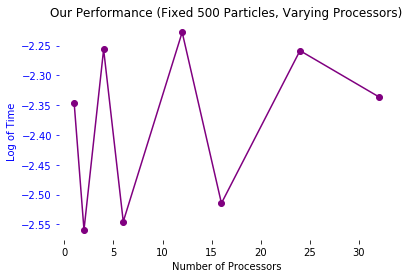
\includegraphics[width = 0.65\textwidth]{500_fixed_particles_varying_processor.png}
  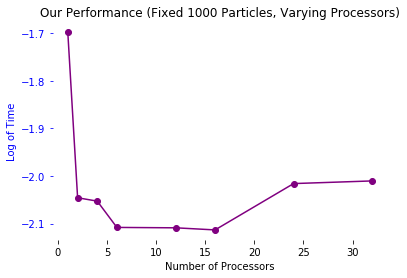
\includegraphics[width = 0.65\textwidth]{1000_fixed_particles_varying_processor.png}
  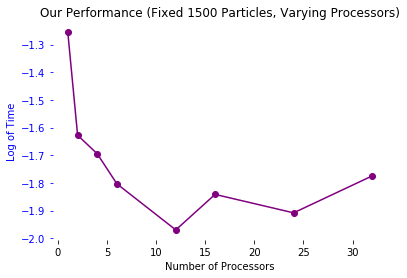
\includegraphics[width = 0.65\textwidth]{1500_fixed_particles_varying_processor.png}
\end{figure}


\begin{figure}[h]
  \caption{Varying Particle Size with Processor}
  \centering
    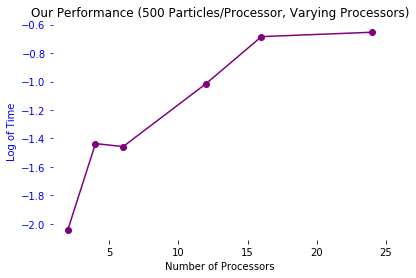
\includegraphics[width = 0.65\textwidth]{500_varying_particles_varying_processor.png}
  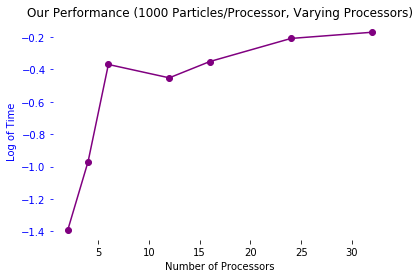
\includegraphics[width = 0.65\textwidth]{1000_varying_particles_varying_processor.png}
  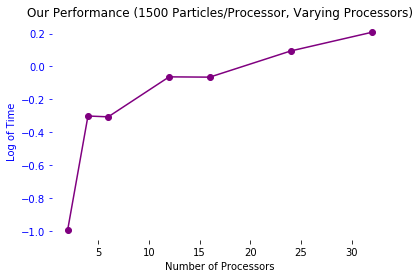
\includegraphics[width = 0.65\textwidth]{1500_varying_particles_varying_processor.png}
 
\end{figure}

\clearpage
\subsection{Doing Better?}
We attempted other variants of MPI, including as mentioned, different shapes for the "sector" used by each processor. We may possibly see different results if, for example, processors which are assigned to the outer blocks of the grid are larger, specifically because particles bounce back from the wall on the outer edge, requiring less communication. 
\\ \\
Another optimization considered is the communication architecture used as well - we found that including a master processor which controls the synchronization of the worker processors resulted in a slow down. It is possible that we could, instead of enforcing every worker processor to signal all of the other worker processors its completion, we divide the grid into e.g. 2 groups, with 2 masters - this way all processors belonging to a group may only signal his completion to the corresponding master, and allow synchronization between the two masters. This setting would be more appropriate for 2 dense regions that are not connected well. 
% --------------------------------------------------------------
%     You don't have to mess with anything below this line.
% --------------------------------------------------------------
 
\end{document}
